\documentclass[11pt, a4paper]{article}

\usepackage{graphicx}
\usepackage{fullpage}

\begin{document}
\title{FYSS360 Numerical exercise}
\author{Sakari Kapanen}
\date{\today}
\maketitle

A single particle electron model was used to estimate the loss cone of electrons in an ECR ion source. It is also a demonstration of the confinement of electrons (and ions) in a magnetic bottle formed by the generated solenoid and hexapole magnetic fields.

The on-axis solenoid field $B_z(r=0, z)$ and the hexapole field $B(x, y)$ were plotted (figures~\ref{fig:solenoidb} and~\ref{fig:hexapoleb}).
\begin{figure}
    \centering
    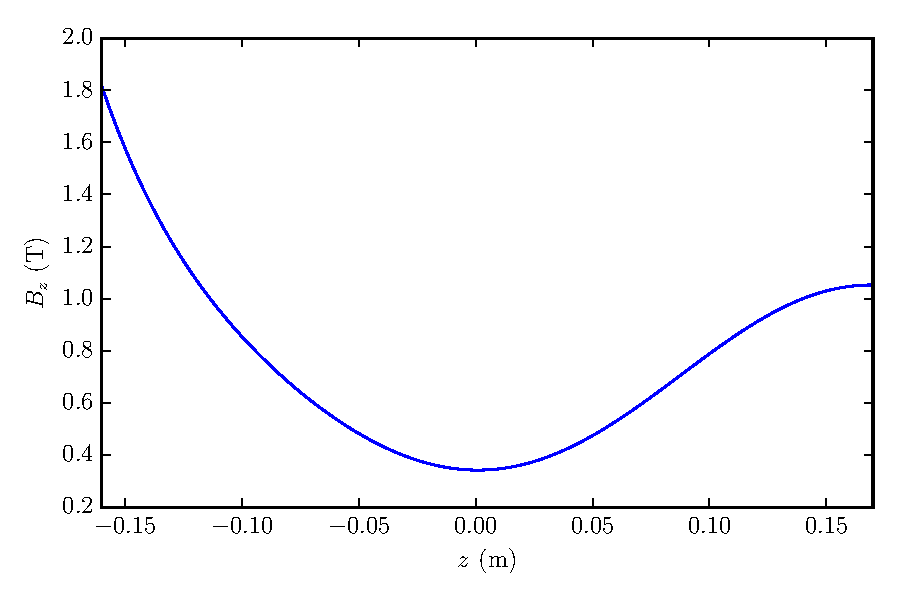
\includegraphics[width=\textwidth]{output/solenoid_B_onaxis.pdf}
    \caption{Solenoid on-axis magnetic field $B_z(r=0, z)$.}
    \label{fig:solenoidb}
\end{figure}
\begin{figure}
    \centering
    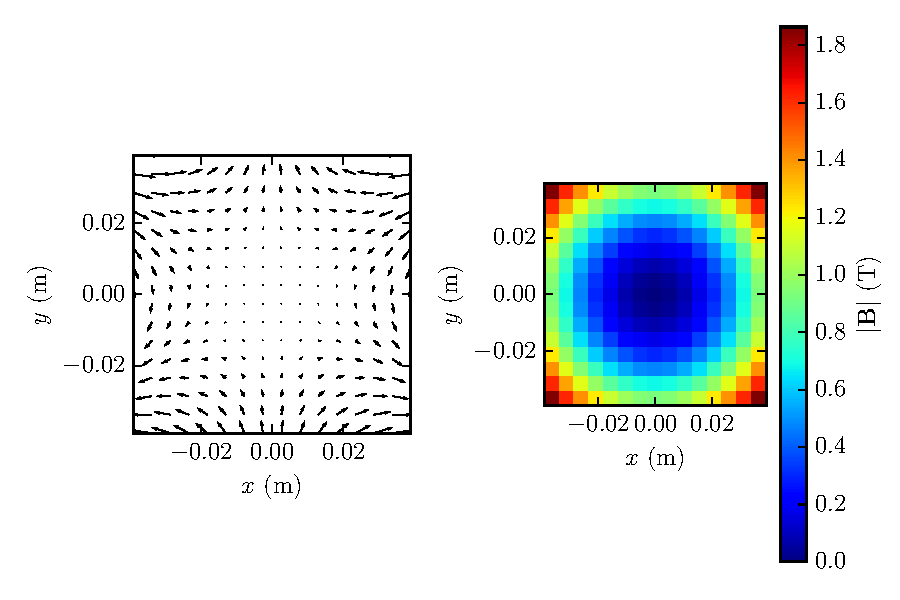
\includegraphics[width=\textwidth]{output/hexapole_B.pdf}
    \caption{The direction and magitude of the hexapole B field.}
    \label{fig:hexapoleb}
\end{figure}

\end{document}

